%%
%% Bioinformatics Applications Note --- working manuscript.
%%
%% LAYOUT NOTE: Bioinformatics' own LaTeX class (bioinfo.cls) is distributed
%% behind the OUP author-guidelines login, so this file uses a two-column
%% article layout that approximates the published page geometry. That keeps the
%% two-page limit verifiable now; at submission replace the preamble with the
%% official class and keep the body commands unchanged. See README.md.
%%
%% NUMBER PROVENANCE: every quantitative claim below is copied from
%% benchmarks/results/paper_data.json, timing_43variants.json and
%% download_throughput.json. paper/BIOINFORMATICS_PLAN.md (section 4) holds the
%% claim -> artifact-key map.
%%
\documentclass[10pt,twocolumn,letterpaper]{article}

\usepackage[T1]{fontenc}
\usepackage[utf8]{inputenc}
\usepackage{lmodern}  % the official OUP class sets its own fonts
\usepackage[margin=0.70in,columnsep=0.26in]{geometry}
\usepackage{graphicx}
\usepackage{booktabs}
\usepackage{amsmath}
\usepackage[hidelinks]{hyperref}
\usepackage{xcolor}
\usepackage{caption}
\usepackage{microtype}

\captionsetup{font=small,labelfont=bf,skip=4pt}
\setlength{\parskip}{0pt}
\pagestyle{empty}

% Placeholder author block --- replace before submission (ORCID required by OUP).
\newcommand{\authornote}{%
  \begin{center}
  \footnotesize\textbf{[Author list and affiliations to be inserted; ORCID iDs required]}\\[2pt]
  \textit{Correspondence: [email]}
  \end{center}}

\title{\vspace{-1.6em}\bfseries lit-acquisition: multi-source, multilingual biomedical
literature acquisition with citation-graph traversal\vspace{-0.4em}}

\author{}
\date{}

\begin{document}
\maketitle
\thispagestyle{empty}
\vspace{-3.2em}
\authornote
\vspace{-0.6em}

\section*{Summary}
Comprehensive literature review is essential for clinical variant
interpretation, yet most retrieval tools query one database and are
English-centric. \textbf{lit-acquisition} unifies \textbf{19 literature
channels} --- 15 federated search backends plus PubMed, Semantic Scholar,
ClinicalTrials.gov and Zenodo services --- behind one interface, and adds
LLM-based cross-lingual query translation and citation-graph traversal. On an
exploratory reference set of \textbf{43 genetic variants (822 papers)} that is
heuristically annotated, not expert-verified, and whose candidate pool overlaps
the evaluated system, the end-to-end pipeline raises PubMed-only set recall from
\textbf{0.269 to 0.467} (+0.198; bootstrap 95\% CI [+0.123, +0.269];
Holm-adjusted $p=0.0002$), and recovers \textbf{21 of 24} annotated
German/French papers where every English-only baseline finds at most one. The
toolkit ships as a lightweight API-only edition and an LLM-enhanced agent
edition (v0.5.0, MIT).

\noindent\textbf{Availability:} \texttt{pip install lit-acquisition} ~$\cdot$~
\url{https://github.com/lanshi17/lit-acquisition} ~$\cdot$~ MIT licence.\\
\noindent\textbf{Contact:} [corresponding author email]

\section{Introduction}
Variant classification under the ACMG/AMP framework requires the assembler to
marshal published evidence: case reports, functional assays and segregation
data that together support criteria such as PS3 or PVS1 \cite{richards2015}.
That evidence is scattered across dozens of databases, publishers, preprint
servers and languages, and it is growing faster than any curator can read.

Existing tooling leaves three gaps. \emph{Single-source} interfaces (PubMed,
Europe PMC) see only their own index, while a variant's literature is split
across Crossref-registered journals, PMC deposits and non-indexed venues
\cite{sayers2024,ferguson2021,visser2021}. \emph{Language}: clinically decisive
case reports appear in German, French, Japanese or Russian venues that
English-only queries cannot reach. \emph{Citation structure}: keyword search
misses papers whose titles omit the variant, although they are one hop away.
Commercial curation platforms cover parts of this, but they are closed and
expensive; no open toolkit combines all three behind one scriptable
interface.

We present \textbf{lit-acquisition}, an open-source Python toolkit that closes
those three gaps in one pipeline, and we report an exploratory coverage
evaluation against a Pub\-Med-centred reference set with an explicit account of
what that reference set can and cannot support.

\section{Implementation}
\subsection*{Pipeline}
Acquisition runs in three phases (Figure~\ref{fig:overview}A). \emph{Search}
fans out across 19 channels --- 15 pure-Python \texttt{httpx} backends
(Crossref, OpenAlex, Europe PMC, PMC, DOAJ, J-STAGE, CiNii, SciELO, BASE, CORE,
OpenAIRE, arXiv, bioRxiv, medRxiv, Unpaywall) plus PubMed, Semantic Scholar,
ClinicalTrials.gov and Zenodo clients --- with a shared connection
pool, per-provider deadlines, health-aware ordering and a circuit breaker;
results are deduplicated on DOI, PMID and normalised title.
\emph{Download} resolves open access only (DOI$\rightarrow$Unpaywall,
PMCID$\rightarrow$Europe PMC render, then direct URL) with SSRF validation on
every redirect hop and streamed size caps. \emph{Gate / rank} applies
token-overlap ranking (CJK-bigram aware) and, in the agent edition, a
cross-encoder rerank \cite{chen2024} plus an LLM relevance gate.

\subsection*{Multilingual routing and citation traversal}
The agent edition translates the query into six languages
(en/zh/ja/de/fr/ru) with domain-aware prompts that preserve gene symbols and
HGVS nomenclature, then routes each language to the channels that index it; the
recorded run used Qwen2.5-72B-Instruct at temperature 0.2, with the prompt hash
stored in the run manifest \cite{qwen2024}. From a seed DOI the toolkit
additionally walks Semantic Scholar citation and reference edges breadth-first
(depth and fan-out configurable; depth 1, 20 papers here), deduplicating
against keyword results \cite{kinney2023}.

\subsection*{Packaging}
Python $\geq$3.12, on \texttt{httpx}, \texttt{pydantic}, \texttt{loguru} and
\texttt{pymupdf}. \texttt{pip install lit-acquisition} installs the lite
edition; \texttt{lit-acquisition[agent]} adds the OpenAI-compatible client for
translation, gating and reranking, which the lite edition replaces with coded
warnings (\texttt{CONFIG\_MISSING}, \texttt{PROVIDER\_HTTP\_429},
\texttt{TIMEOUT}, \dots) and a purely heuristic pipeline.

\section{Results}
\subsection*{Reference set and protocol}
The reference set holds 43 clinically actionable variants (BRCA1, TP53, CFTR,
HFE, \dots) and 822 papers, built by an automated heuristic protocol scoring
gene, variant token, disease keyword and publication type. It is \emph{not}
expert-verified and its candidate pool was drawn from channels that overlap the
evaluated system, so every number below is a \emph{relative} coverage
comparison, not a clinical retrieval-quality estimate. Only German (13 papers)
and French (11) carry non-English annotations; 305 have no language label. We
compare four configurations at a uniform 100-candidate budget with a strictly
nested ablation, testing paired differences by two-sided Wilcoxon signed-rank
under Holm--Bonferroni correction over a pre-declared family of eight tests
(10{,}000 bootstrap resamples, seed 42).

\begin{table}[t]
\centering
\footnotesize
\caption{Relative coverage over 43 variants (macro means). M4n is the nested
ablation: frozen M3 ranking plus citation-graph items.}
\label{tab:main}
\begin{tabular}{lcccc}
\toprule
 & SetRecall & Recall@20 & nDCG@20 & Relevant \\
\midrule
M1 PubMed-only        & 0.269 & 0.171 & 0.205 & 213 \\
M2 multi-source       & 0.472 & 0.153 & 0.164 & 373 \\
M3 + translation      & 0.465 & 0.276 & 0.301 & 392 \\
M4n + citation        & \textbf{0.467} & \textbf{0.276} & \textbf{0.301} & \textbf{394} \\
\bottomrule
\end{tabular}
\end{table}

\subsection*{Federation is the main effect}
The pipeline significantly improves coverage over PubMed-only:
SetRecall $+0.198$ (95\% CI $[+0.123,+0.269]$; $p_{\text{Holm}}=0.0002$;
matched-pairs rank-biserial $r=0.74$), and shallow ranking improves as well
(Recall@20 $+0.105$, $p_{\text{Holm}}=0.016$; nDCG@50 $+0.162$,
$p_{\text{Holm}}=0.0004$). Decomposing the gain shows that \emph{federation}
carries it ($+0.203$ over M1, $p_{\text{Holm}}=0.0001$): translation and
citation are set-level neutral ($p_{\text{Holm}}=1.0$ in both pairwise
contrasts), and citation traversal costs list precision
($-0.011$ Precision@Retrieved, $p_{\text{Holm}}=1.9\times10^{-6}$).

\subsection*{Multilingual recovery}
Translation does not raise aggregate set recall, but it changes \emph{which}
papers are reachable: M3/M4n recover 21 of the 24 annotated German and French
reference papers (11/13 German, 10/11 French), whereas every English-only
baseline --- including multilingual dense retrieval --- recovers at most one.
This is the clearest practical argument for language-aware routing.

\subsection*{Citation traversal and single-channel baselines}
Across all 43 variants citation traversal contributes two relevant papers that
keyword search did not rank, one appearing in no keyword list at all (V002
BRCA1 c.5266dupC; V035 HFE p.C282Y) --- a bounded complementary channel, not a
headline gain. Against six 2025--2026 single-channel techniques (dense
retrieval, cross-encoder reranking, hybrid BM25+dense+rerank, LLM query
expansion, agentic two-round search, multilingual dense) the pipeline is
significantly better than five; the strongest, hybrid BM25+dense+rerank
(0.421), stays below M4n (0.467) but not significantly so
(raw $p=0.35$, Holm-adjusted $p=1.00$). Four of the six only reorder the same PubMed pool
(mean 80.7 candidates) and are identical to M1 on set recall by construction.

\subsection*{Cost}
In the 43-variant session the composed full pipeline took a median of 28.65\,s
per variant (p90 44.61\,s) at a 100-candidate budget, including provider
back-off. A separate four-variant download measurement landed 18 PDFs from 187
candidates: 3.99 PDFs/min end-to-end, 9.6\% candidate-to-PDF, 15.06\,s per PDF,
peak RSS 85.7\,MB. Downloading requires \texttt{LIT\_UNPAYWALL\_EMAIL};
without it every DOI$\rightarrow$OA route is skipped.

\section{Discussion}
lit-acquisition combines multi-source federation, cross-lingual translation and
citation traversal in one reproducible pipeline, and its coverage gain over
PubMed-only is statistically robust on this reference set. Two limitations
matter. The reference set is heuristically annotated with an overlapping
candidate pool, so the deltas measure relative reach, not clinical
completeness; expert re-annotation is in progress. And the cost is real
(~29\,s per variant, ~4 PDFs/min): adequate for curation-scale batches, not for
interactive search. Future work targets embedding-based semantic search,
adaptive traversal depth and integration with variant databases such as ClinVar
\cite{landrum2018}.

\section*{Funding}
[To be completed.]

\section*{Conflict of interest}
None declared.

\section*{Acknowledgements}
[To be completed.] We thank the operators of all 19 public APIs used here.

\begin{figure*}[t]
\centering
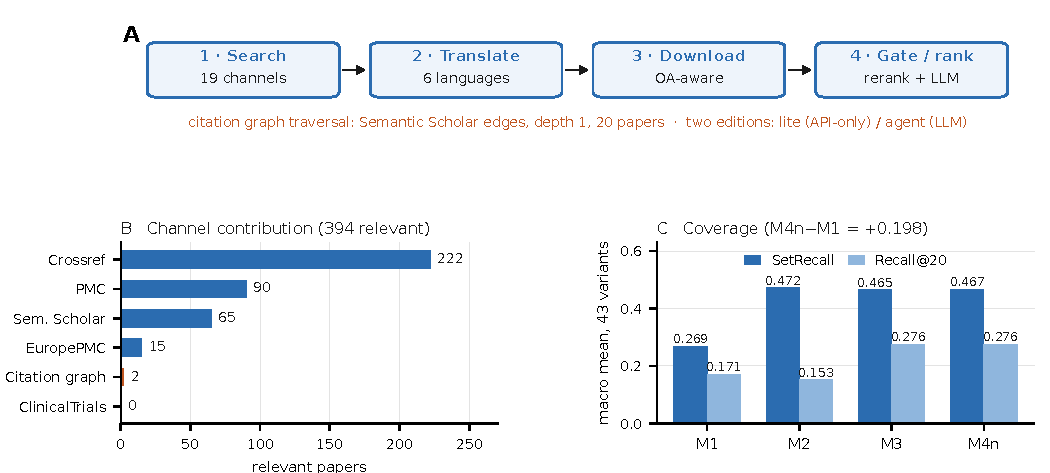
\includegraphics[width=\textwidth]{figure1.pdf}
\caption{\textbf{lit-acquisition at a glance.} \textbf{(A)}~The three-phase
pipeline across 19 channels and the two editions. \textbf{(B)}~Relevant
reference papers per channel in the nested M4 run (first-seen attribution after
deduplication). \textbf{(C)}~Macro-mean SetRecall and Recall@20 over 43
variants for M1 PubMed-only, M2 multi-source, M3 +translation and M4n +citation
(nested); M4n$-$M1 $=+0.198$ (95\% CI $[+0.123,+0.269]$,
$p_{\text{Holm}}=0.0002$).}
\label{fig:overview}
\end{figure*}

\begin{thebibliography}{99}
\scriptsize
\setlength{\itemsep}{-1pt}
\setlength{\parskip}{0pt}

\bibitem{richards2015} Richards S, Aziz N, Bale S, \textit{et al.} Standards
and guidelines for the interpretation of sequence variants. \textit{Genet Med}
2015;\textbf{17}:405--424.

\bibitem{landrum2018} Landrum MJ, Lee JM, Benson M, \textit{et al.} ClinVar:
improving access to variant interpretations and supporting evidence.
\textit{Nucleic Acids Res} 2018;\textbf{46}(D1):D1062--D1067.

\bibitem{sayers2024} Sayers EW, Beck J, Bolton EE, \textit{et al.} Database
resources of the National Center for Biotechnology Information.
\textit{Nucleic Acids Res} 2024;\textbf{52}(D1):D33--D43.

\bibitem{ferguson2021} Ferguson C, Ara\'ujo D, Faulk L, \textit{et al.} Europe
PMC in 2020. \textit{Nucleic Acids Res} 2021;\textbf{49}(D1):D1507--D1514.

\bibitem{visser2021} Visser M, van Eck NJ, Waltman L. Large-scale comparison of
bibliographic data sources. \textit{Quant Sci Stud} 2021;\textbf{2}(1):20--41.

\bibitem{priem2022} Priem J, Piwowar H, Orr R. OpenAlex: a fully-open index of
scholarly works, authors, venues, institutions, and concepts.
\textit{arXiv:2205.01833} 2022.

\bibitem{kinney2023} Kinney R, Anastasiades C, Authur R, \textit{et al.} The
Semantic Scholar Open Data Platform. \textit{arXiv:2301.10140} 2023.

\bibitem{robertson2009} Robertson S, Zaragoza H. The probabilistic relevance
framework: BM25 and beyond. \textit{Found Trends Inf Retr}
2009;\textbf{3}(4):333--389.

\bibitem{karpukhin2020} Karpukhin V, O\u{g}uz B, Min S, \textit{et al.} Dense
passage retrieval for open-domain question answering. In: \textit{Proc EMNLP}
2020:6769--6781.

\bibitem{nogueira2019} Nogueira R, Cho K. Passage re-ranking with BERT.
\textit{arXiv:1901.04085} 2019.

\bibitem{chen2024} Chen J, Xiao S, Zhang P, \textit{et al.} BGE M3-Embedding:
multi-lingual, multi-functionality, multi-granularity text embeddings through
self-knowledge distillation. \textit{arXiv:2402.03216} 2024.

\bibitem{qwen2024} Yang A, Yang B, Zhang B, \textit{et al.} Qwen2.5 technical
report. \textit{arXiv:2412.15115} 2024.

\end{thebibliography}


\end{document}
